\section{Risikoanalyse}
\begin{figure}[H]
	\centering
	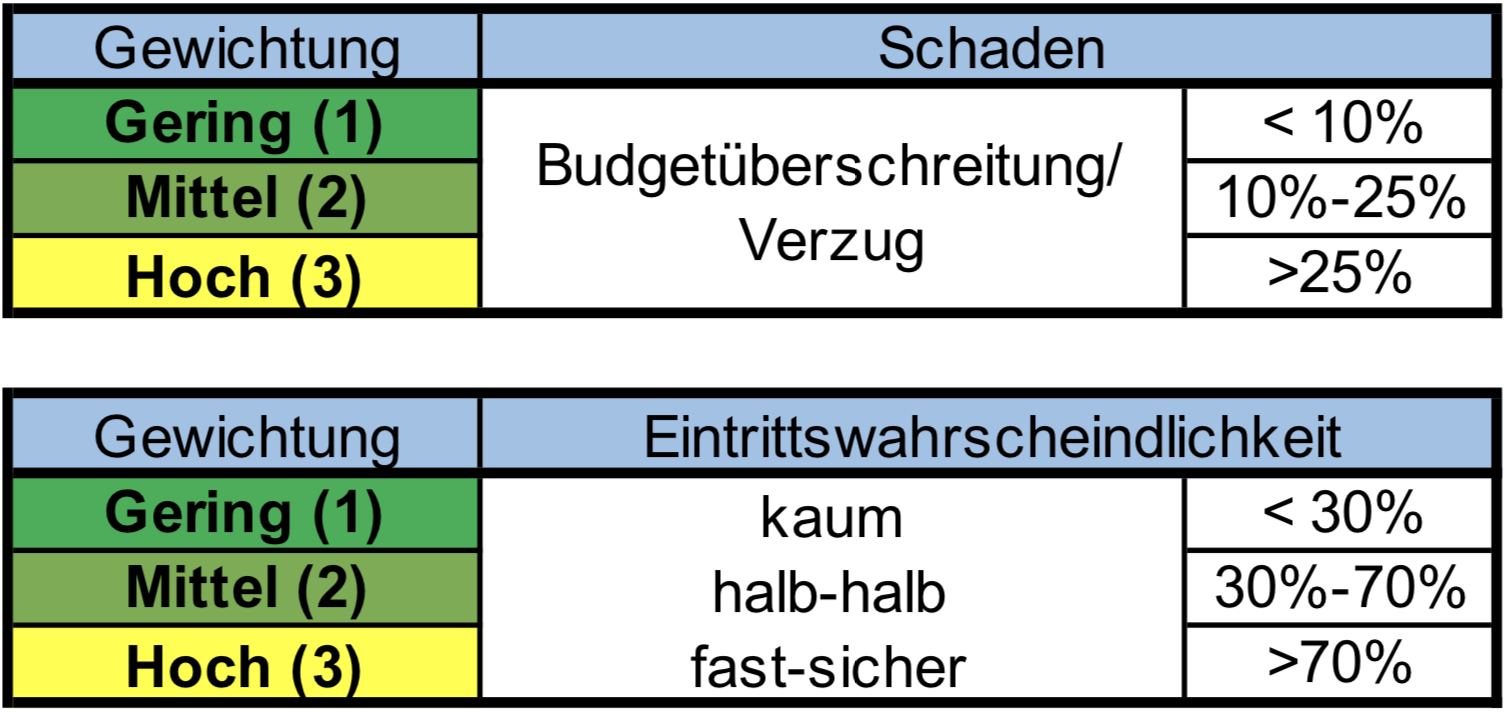
\includegraphics[width=14cm]{Gewichtung_P2.png}
	\label{fig:Gewichtung}
\end{figure}

\newpage



\begin{figure}[H]
\centering
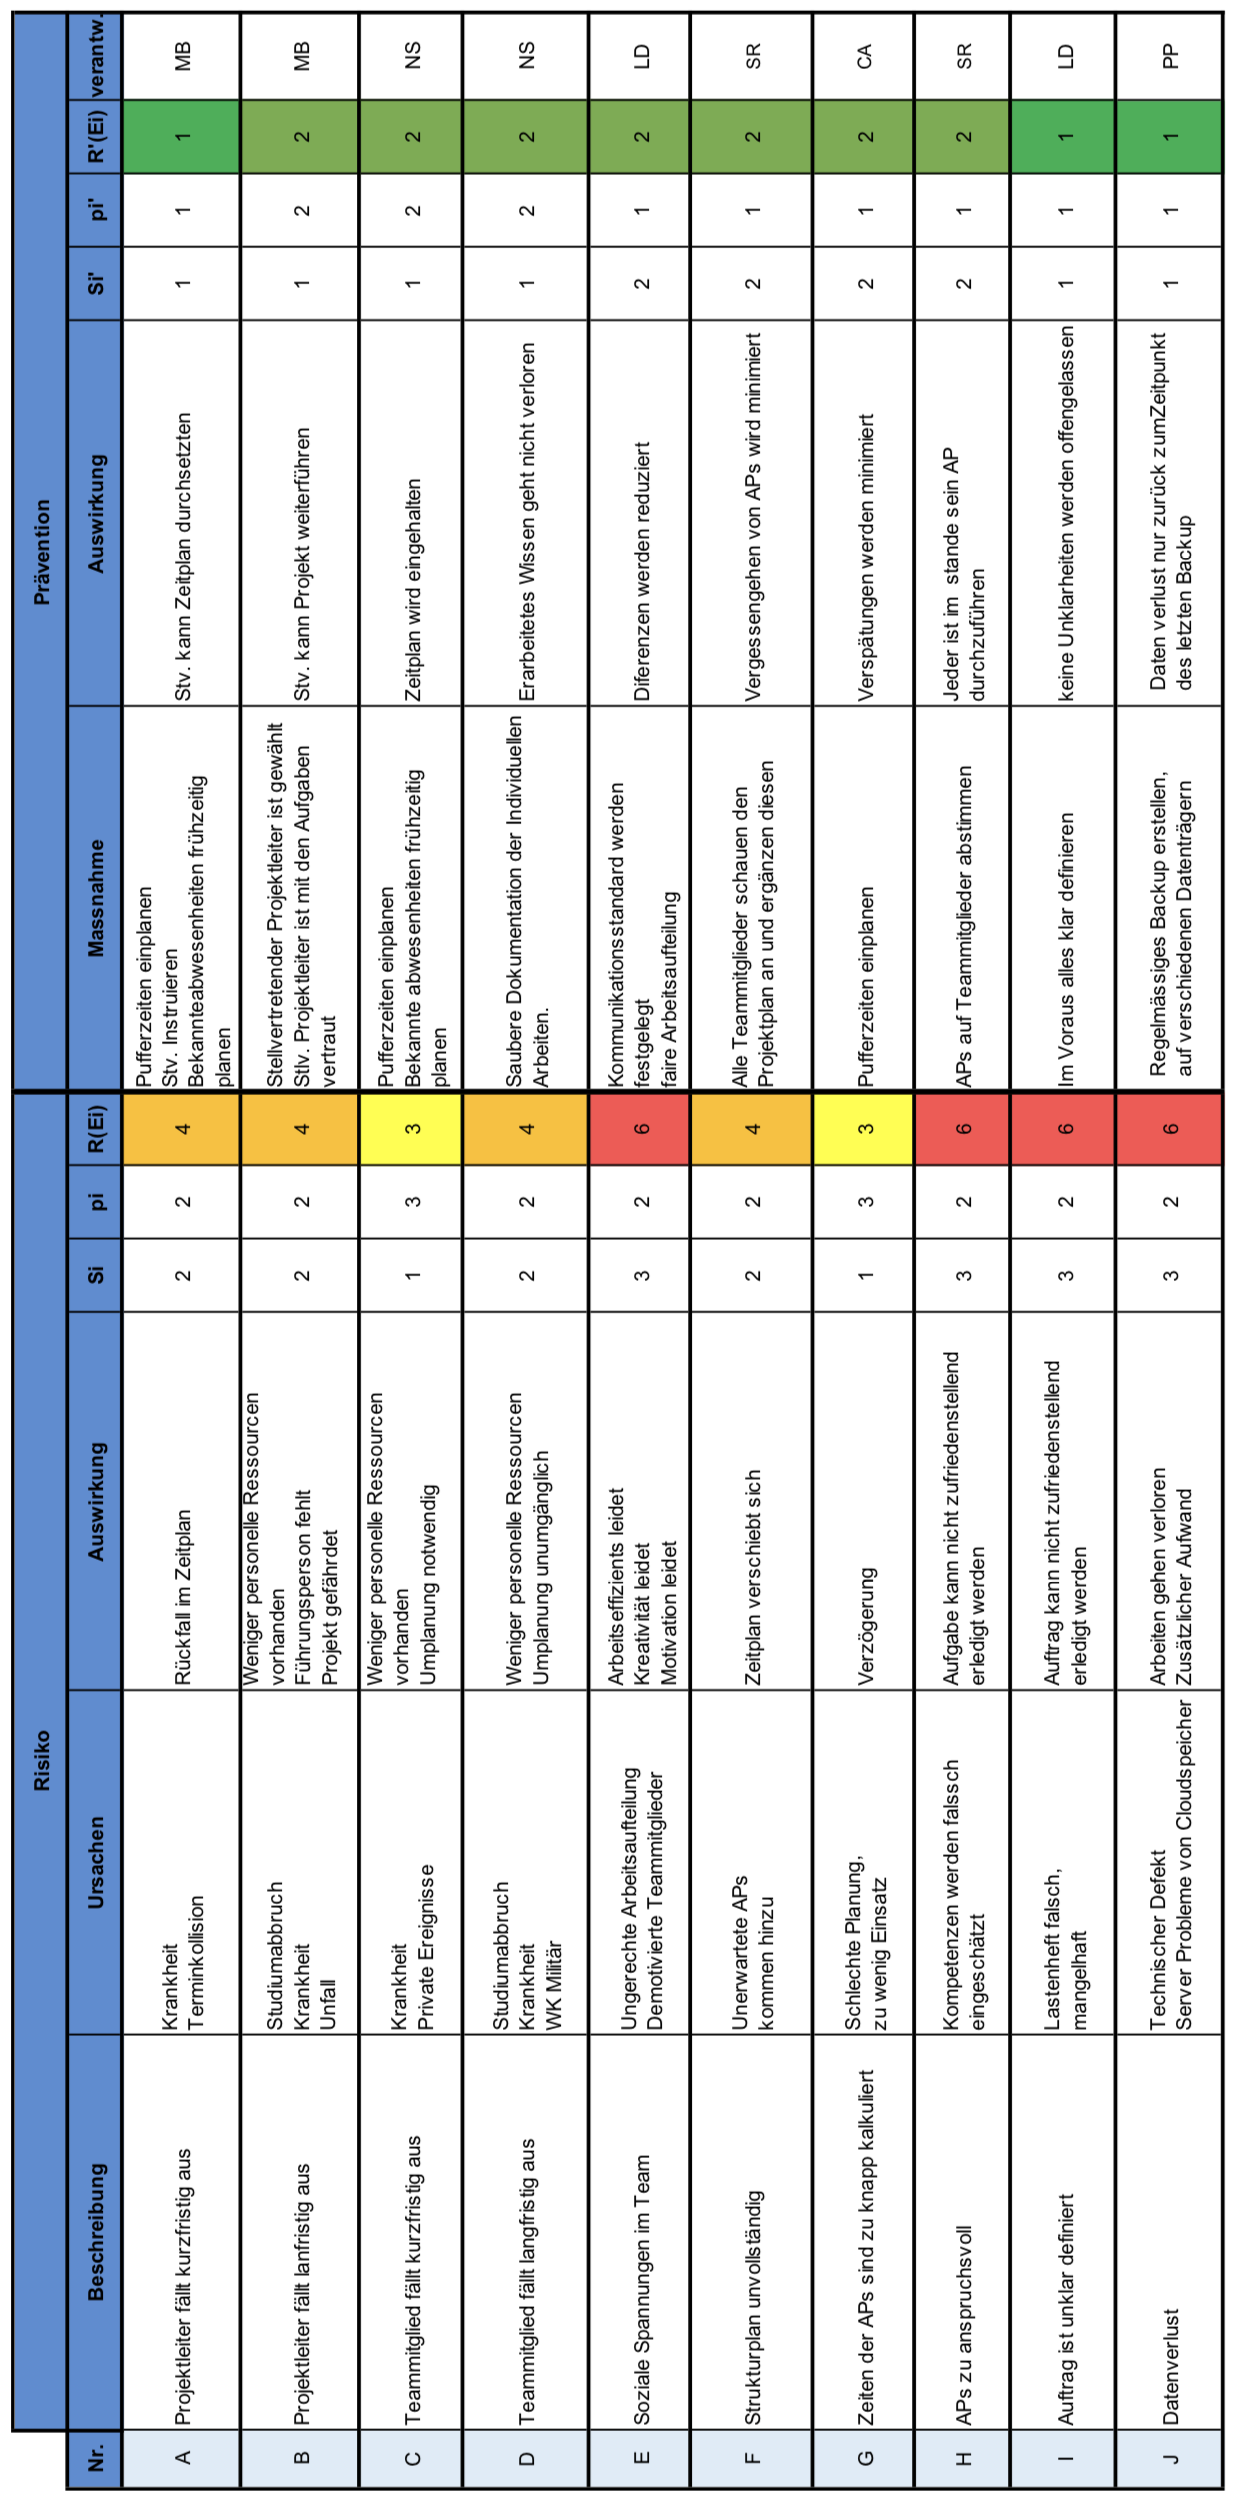
\includegraphics[width=12.5cm]{Risikotabelle_P2.png}
\label{fig:Risikotabell}
\end{figure}

\newpage
\begin{figure}[H]
	\centering
	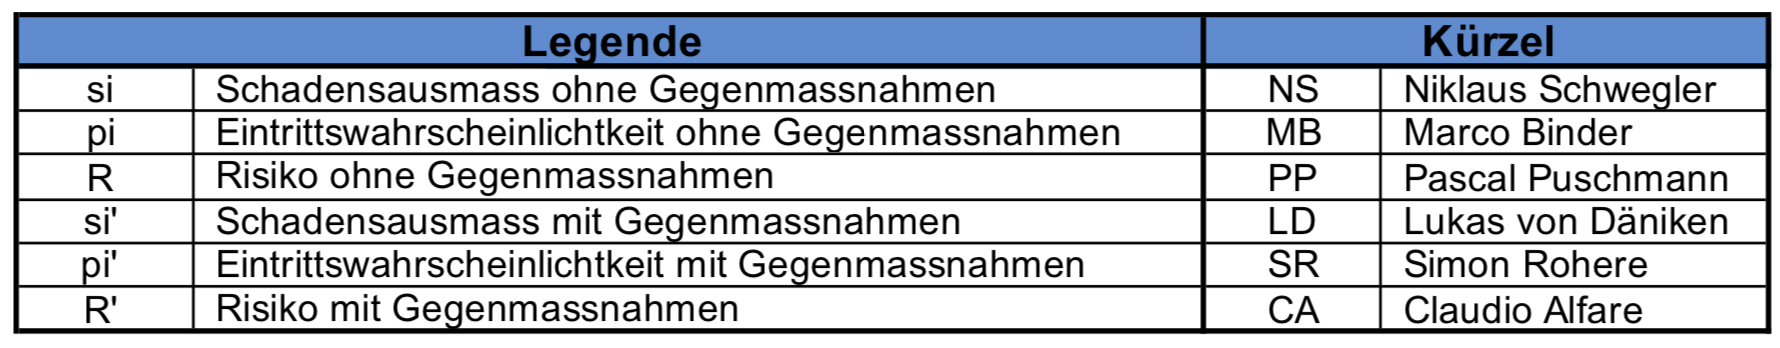
\includegraphics[width=14cm]{Legende_P2.png}
	\label{fig:Tabelle}
\end{figure}
Um auf Risiken vorbereitet zu sein, haben wir obige Risikotabelle erstellt. In dieser listen wir die möglichen Gefahren auf und nennen Präventionsmassnahmen, um sowohl die Eintrittswahrscheinlichkeit(Pi), als auch die Auswirkungen(Si) zu minimieren.\\
Auf der folgenden Risikomap sind alle Gefahren mit und ohne Prävention graphisch dargestellt.

\begin{figure}[H]
	\centering
	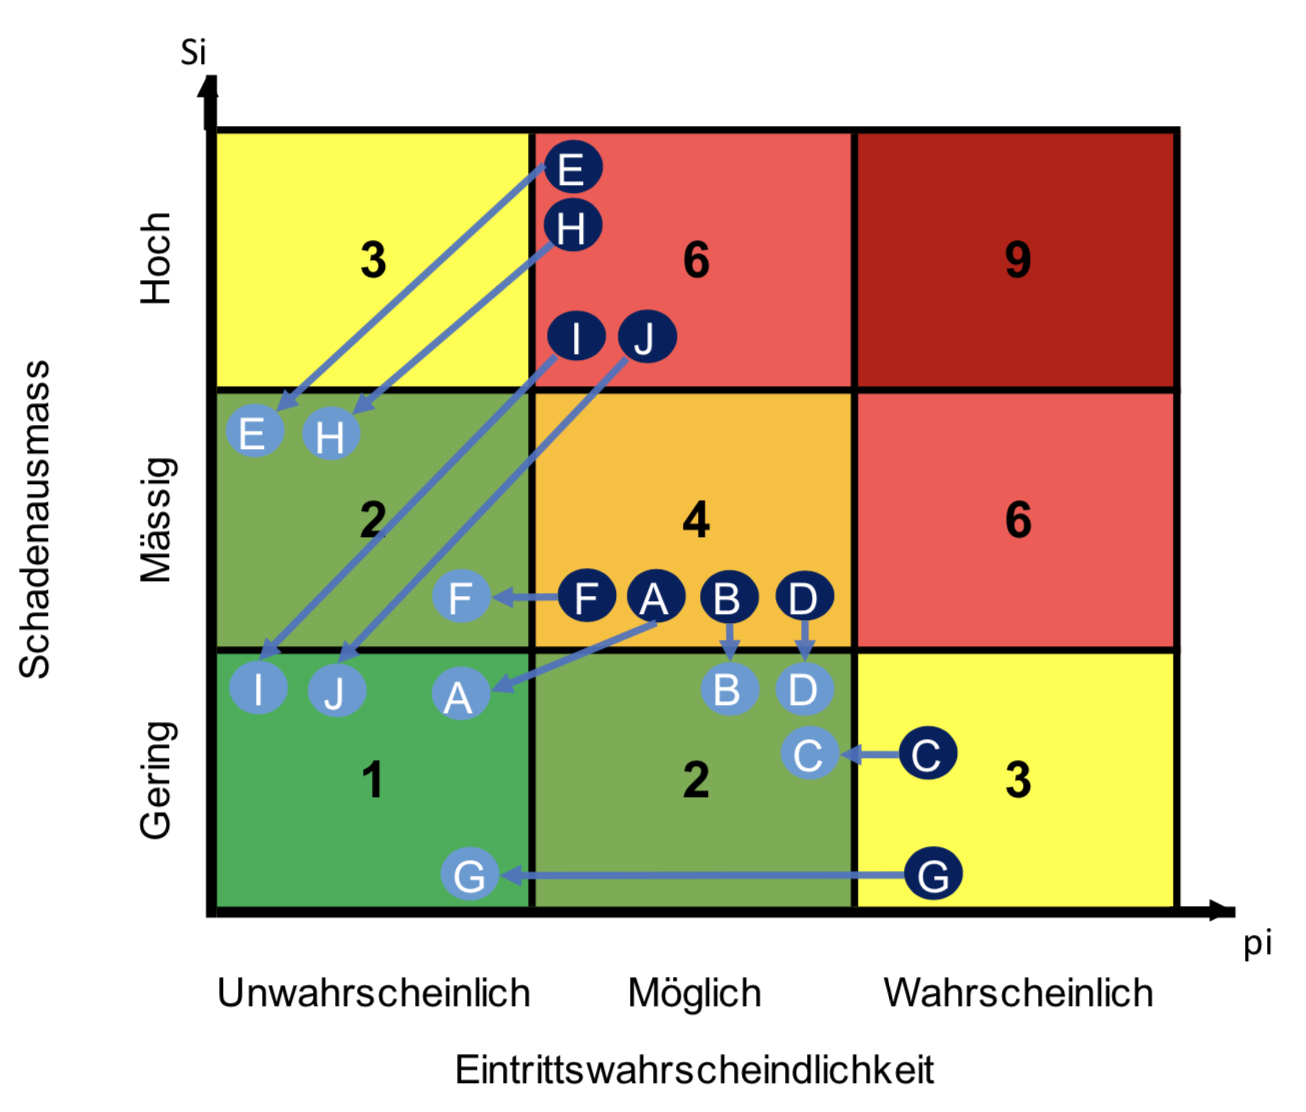
\includegraphics[width=14cm]{Matrix_verschiebung_P2.png}
	\label{fig:Matrix_verschiebung}
\end{figure}


\begin{figure}[H]
	\centering
	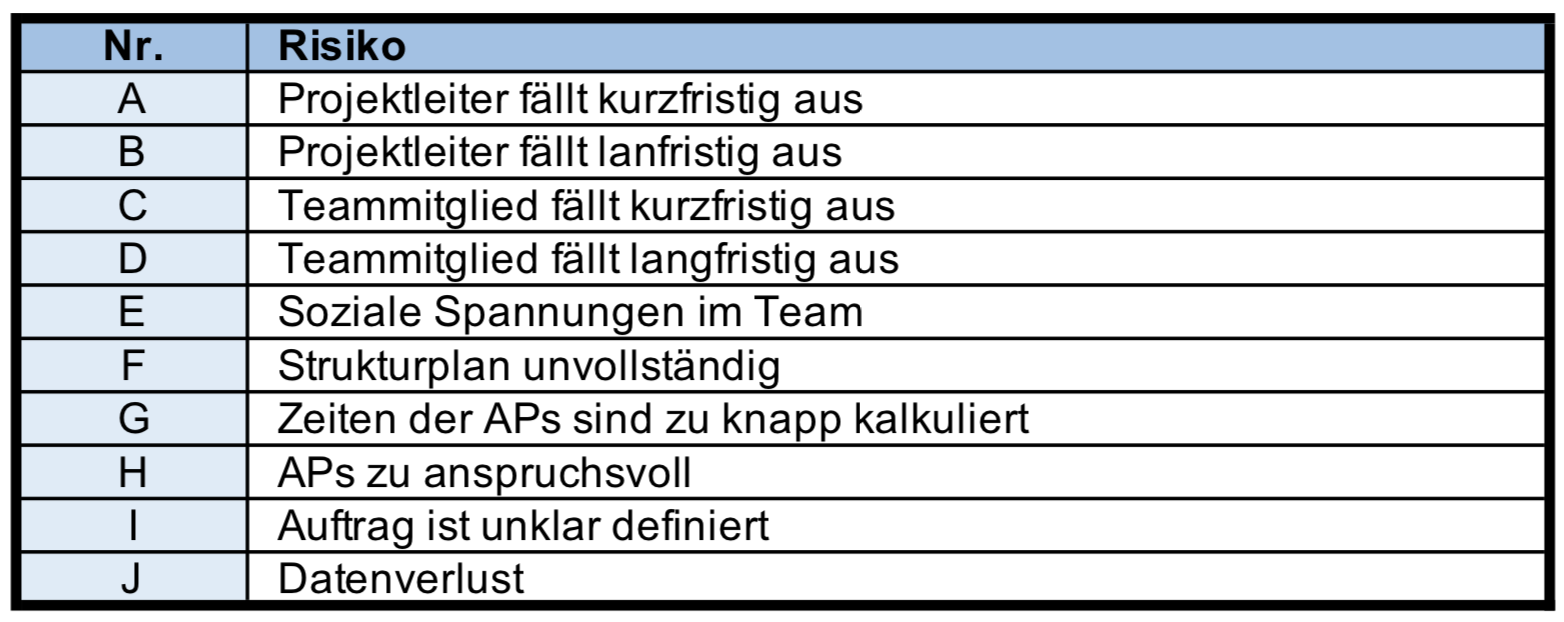
\includegraphics[width=14cm]{Risikouebersicht_P2.png}
	\label{fig:Risikoüebersicht}
\end{figure}
